\documentclass[a4paper,12pt]{article}

% \usepackage{ucs}
\usepackage[utf8]{inputenc}
\usepackage{amsmath}
\usepackage{amsfonts}
\usepackage{amssymb}
\usepackage{caption}
\usepackage{mathpazo}
\usepackage{makeidx}
\usepackage{multicol}
\usepackage{fontenc}
\usepackage{graphicx}
\usepackage{listings}
\usepackage{float}
\lstset{breaklines=true}
\lstset{basicstyle=\ttfamily}
\lstset{framesep=10pt}
\usepackage{lscape}
\usepackage[top=1in,bottom=1in,right=1in,left=1in]{geometry}
\usepackage{float}

\usepackage[dvips]{hyperref}

\author{Paul Korir and Cathal Seoighe}
\title{\textbf{MaLTE: Machine Learning of Transcript Expression}\\\textit{An \textsf{R} Package Implementing the MaLTE Framework}}
\date{}

\makeindex
\begin{document}
\maketitle

\tableofcontents

\newpage

% \begin{abstract}
% MaLTE is a novel approach to gene and transcript expression prediction that uses a supervised learning approach to achieve performance superior to conventional microarray summarisation. It learns from a gold standard how best to use fluorescence probe intensity values. This leads to more accurate and absolute expression estimates as well as an simple facility to obtain expression estimates for individual transcript isoforms.
% \end{abstract}

\section{Introduction}
\label{introduction}
Quantification of oligonucleotide expression microarrays involves assembling probe fluorescence intensities from sets of probes into a single gene or transcript expression measure, a process referred to as \textit{summarisation} \cite{irizarry2003summaries}. There is a long list of summarisation algorithms \cite{irizarry2006comparison} most of which suffer from two main problems: they produce relative, as opposed to absolute, estimates \cite{irizarry2005multiple, fu2009estimating} and they are oblivious to the abundance of individual transcript abundances \cite{malone2011microarrays}. 

The \textsf{MaLTE} framework supplements conventional algorithms with a supervised learning approach between a gold standard probe fluorescence intensities. As a framework the various components may be modified or entirely overhauled; it is not restricted to the learning algorithms used in the \textsf{R} \textsf{MaLTE} package (conditional random forest (CRF) and quantile regression random forest (QRF)). Currently, we use RNA-Seq as the gold standard HTS quantification technique. Figure \ref{fig:schematic} below shows a schematic of the \textsf{MaLTE} framework. Learning occurs for each gene independently though only one gene is illustrated. For gene expression, \textsf{MaLTE} incorporates simple feature selection by picking the best 15 probes that correlate with the expression in the gold standard.

\begin{figure}[H]
\centering
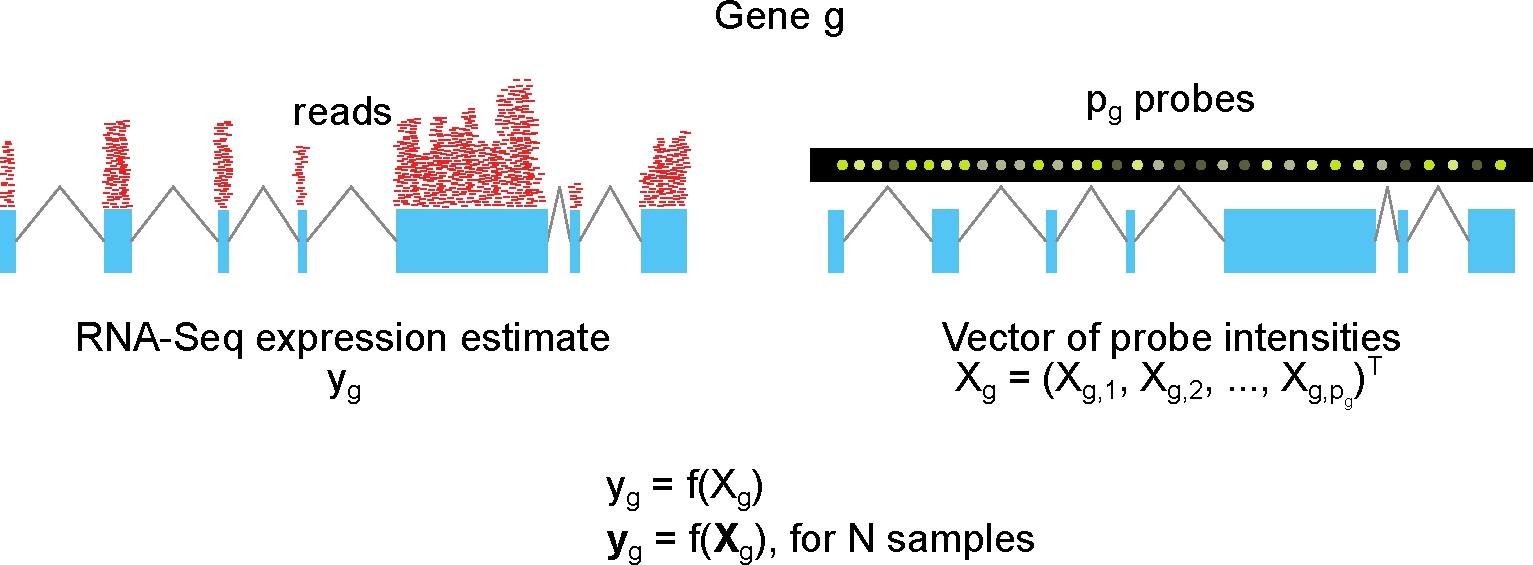
\includegraphics[width=\columnwidth]{schematic.pdf}
\caption{\textbf{Schematic of the MaLTE framework.} A supervised learning algorithm is used to learn the relationship between a gold-standard (RNA-Seq) and probe fluorescence intensities. The learned model may then be applied to a new set of probes.}
\label{fig:schematic}
\end{figure}

This approach overcomes the two main setbacks of conventional algorithms. It transforms expression estimates onto an absolute scale thus dramatically improving the within-sample correlations and naturally extends to predicting expression of individual transcript isoforms by training on the multiple responses of individual transcript isoforms. Moreover, \textsf{MaLTE} leads to substantial improvements in cross-sample correlations, which increases statistical power for biological analyses. Finally, a tree-based learning introduces an easy way to filter out poorly-predicted genes through the use of out-of-bag estimates.

This documents describes how to use the \textsf{R} \textsf{MaLTE} package. It begins with a description on how to get and install the package. It then outlines the two main ways in which the package may be used: \textit{gene expression prediction (GEP)} and \textit{transcript isoform expression prediction (TIEP)}. It concludes with a description on how to filter and collate expression predictions for downstream analyses. It also provides a tentative roadmap for future development as well as a detailed description on how the \textsf{MaLTE} package is built. Bug reports, comments and suggestions are welcome through \href{mailto:paul.korir@gmail.com}{paul.korir@gmail.com}.

\section{Conventions Used}
\label{conventions}
\begin{itemize}
\item Array data used here corresponds to that from \textit{Affymetrix GeneChip$^{\textregistered}$ Human Exon 1.0 ST} arrays. At present only Affymetrix GeneChip$^{\textregistered}$ Human Exon and Human Gene arrays have been tested using \textsf{MaLTE}.
\item All gene and transcript identifiers are from EnsEMBL (\url{http://www.ensembl.org}).
\item All filenames are written in italics (\textit{filename.txt}), variables in monospace (\texttt{my.var}), and functions in monospace terminated with parentheses (\texttt{my.function()}). Classes are in monospace beginning with a capital letter (\texttt{My.Class}) while corresponding constructors additionally terminate with parentheses (\texttt{My.Class()}). Names of software packages are in sans (\textsf{R}, \textsf{MaLTE}, \textsf{Cufflinks})
\item \textit{High-throughput sequencing (HTS)} refers to \textit{RNA-Seq}.
\item A \textit{map} is a tab-delimited text file with two columns with each column consisting of identifiers/names.
\item The set of samples used for training are called \textit{training samples}. \textit{Test samples} refer to the samples that need to have their gene/transcript expression quantified.
\end{itemize}

\section{System Requirements}
\label{system}
\begin{itemize}
\item \textsf{R} (\texttt{2.14.0} or greater) installed on GNU/Linux: \textsf{MaLTE} has been tested on Scientific Linux version 5
\item \textsf{Python} 2.7 or later
\item \texttt{party} \textsf{R} package
\item \texttt{multicore} \textsf{R} package
\item \texttt{quantrefForest} \textsf{R} package
\end{itemize}

\section{Installation}
\label{installation}
\textsf{MaLTE} may be downloaded from \url{https://github.com/polarise/MaLTE-package}. There are two ways to install \textsf{MaLTE}: via GNU/Linux shell and \textsf{R} shell.

\begin{enumerate}
\item Via GNU/Linux shell
\begin{verbatim}
me@home ~$ R CMD INSTALL MaLTE_<release>.tar.gz
\end{verbatim}

\item Via \textsf{R} shell
\begin{verbatim}
> install.packages( "/path/to/MaLTE_<release>.tar.gz" )
\end{verbatim}
\end{enumerate}

Once installed, \textsf{MaLTE} may be loaded in the \textsf{R} shell as follows:
\begin{verbatim}
> library( MaLTE )
\end{verbatim}

or, quietly:

\begin{verbatim}
> suppressMessages( library( MaLTE ))
\end{verbatim}

\section{Datasets Provided}
\label{datasets}
\begin{enumerate}
\item Sample names files (various provided)
\item HTS data
\item Transcript HTS data
\item Raw microarray data (provided directly from APT)
\item Truncated microarray data (non-essential rows and columns removed)
\item Gene-to-probeset maps for exon array
\item Gene-to-transcript maps
\end{enumerate}

Working with principal components...

\section{Gene Expression Prediction}
\label{gep}
\subsection{Quick Start Guide}
\label{gep:quick}
This section provides a quick introduction to using \textsf{MaLTE}. Detailed instructions incorporating descriptions of the various file and there respective formats is provided in Section \ref{gep:detailed}. It is assumed that the user is in the \textsf{R} shell, the \textsf{MaLTE} library is loaded and the following data files are available: \textit{samples.txt}, \textit{hts\_data.txt}, \textit{ma\_data.txt}, \textit{gene\_probesets.txt}.

\noindent\\
\textbf{Step I:} Provide the location of the file containing a map between sample names on both platforms (RNA-Seq and microarray)
\begin{verbatim}
> samples.fn = paste( system.file( package="MaLTE" ), "data", 
  "samples.txt.gz", sep="/" )
\end{verbatim}

\noindent\\
\textbf{Step II:} Provide the location of the file containing the high-throughput sequencing (RNA-Seq) data
\begin{verbatim}
> hts.fn = paste( system.file( package="MaLTE" ), "data", 
  "hts_data.txt.gz", sep="/" )
\end{verbatim}

\noindent\\
\textbf{Step III:} Provide the location to the file containing quantile-normalised and background corrected fluorescence probe intensities
\begin{verbatim}
> ma.fn = paste( system.file( package="MaLTE" ), "data", 
  "ma_data.txt.gz", sep="/" )
\end{verbatim}

\noindent\\
\textbf{Step IV:} Provide the location of a map showing the probe sets associated with each gene
\begin{verbatim}
> g2p.fn = paste( system.file( package="MaLTE" ), "data", 
  "gene_probesets.txt.gz", sep="/" )
\end{verbatim}

\noindent\\
\textbf{Step V:} Prepare the data into training and test sets
\begin{verbatim}
> prepare.data( samples.fn=samples.fn, ma.fn=ma.fn, hts.fn=hts.fn, 
  g2p.fn=g2p.fn )
\end{verbatim}

\noindent\\
\textbf{Step VI:} Read the data in preparation for the training and test phase
\begin{verbatim}
> tt.ready = read.data( train.fn="train_data.txt.gz", 
  test.fn="test_data.txt.gz" )
\end{verbatim}

\noindent\\
\textbf{Step VII:} Initialise training parameters
\begin{verbatim}
# conditional random forest
> tt.params = TT.Params()

# quantile regression random forest
> tt.params = TT.Params( quantreg=TRUE )
\end{verbatim}

\noindent\\
\textbf{Step VIII:} Train and predict
\begin{verbatim}
> tt.seq = array2seq( tt.ready, tt.params )
\end{verbatim}

\noindent\\
\textbf{Step IX:} Perform out-of-bag (OOB) predictions
\begin{verbatim}
> tt.seq.oob = array2seq.oob( tt.ready, tt.params )
\end{verbatim}

\noindent\\
\textbf{Step X:} Filter based on OOB correlations
\begin{verbatim}
> tt.filtered = oob.filter( tt.seq, tt.seq.oob, thresh=0 )
\end{verbatim}

\noindent\\
\textbf{Step XI:} Get the names of test samples
\begin{verbatim}
> test.names = get.names( samples.fn, test=TRUE )
\end{verbatim}
or 
\begin{verbatim}
> test.names = get.test( samples.fn )   # get test sample names
\end{verbatim}

\noindent\\
\textbf{Step XII:} Aggregate predictions and write output to a text file for downstream analyses.
\begin{verbatim}
> df = get.predictions( tt.filtered, test.names )
> write.table( df, file="filt_preds.txt", col.names=TRUE, row.names=FALSE, 
  quote=FALSE, sep="\t" )
\end{verbatim}

\subsection{Detailed Instructions}
\label{gep:detailed}
Gene expression prediction (GEP) depends on having four input files:
\begin{itemize}
\item \textbf{Sample names.} A map of sample names between both platforms (HTS and array; possibly zipped). An example file is provided with the package (Step I).
\item \textbf{HTS data.} The HTS (RNA-Seq) data in text file (possibly zipped)
\item \textbf{Microarray data.} The microarray probe data (possibly zipped) 
\item \textbf{Gene-to-probeset map.} A map between gene identifiers and probe set identifiers. Probe set identifiers are provided by the array manufacturer as part of the array description.
\end{itemize}

Each file is now described in detail under the following sub-headings: \textit{purpose}, \textit{generic designation}, \textit{header} and \textit{structure}.

\subsubsection{Sample names file}
\label{gep:sample}

\begin{tabular}{rp{12cm}}
\textbf{Purpose} & This file provides a one-to-one map between sample identifiers on both platforms. \\
\textbf{Generic designation} & \textit{samples.txt} OR \textit{samples.txt.gz}; Any suitable name will do but the file name must end either with \textit{*.txt} or \textit{*.txt.gz}. \\
Header & \texttt{hts\textless tab\textgreater ma} \\
Structure & Two-columns separated by a single tab (tab-delimited) \\
  & All sample identifiers must be unique and must exactly correspond to sample names present in the headers of the HTS data and microarray data. For example, microarray probe files will usually have headers with sample names terminated by \textit{*.CEL}; this must be retained in the sample names file. \\
  & Test samples are marked by having an asterisk (\texttt{`*'}) as the first character. Any other row is assumed to be a training sample. \\
  & Test samples may consist of having both HTS and array data. If only test array data is present then the first column must be \texttt{`*NA'}. \\
  & Comments must begin with a pound/hash (\texttt{`\#'}) symbol. \\
\end{tabular}

\subsubsection{HTS data file}
\label{gep:hts}

\begin{tabular}{rp{12cm}}
\textbf{Purpose} & This file provides the HTS expression estimates.\\
\textbf{Generic designation} & \textit{hts\_data.txt} OR \textit{hts\_data.txt.gz} \\
  & Any suitable name will do but the file name must end either with \textit{*.txt} or \textit{*.txt.gz}.. \\
\textbf{Header} & \texttt{gene\_id\textless tab\textgreater Sample01\textless tab\textgreater...\textless tab\textgreater SampleN} \\
\textbf{Structure} & Tab-delimited \\
  & All rows must be unique \\
  & No comments are allowed \\
\end{tabular}

\subsubsection{Microarray data file}
\label{gep:microarray}

\begin{tabular}{rp{12cm}}
\textbf{Purpose} & This file provides the microarray probe intensities. \\
\textbf{Generic designation} & \textit{ma\_data.txt} OR \textit{ma\_data.txt.gz} if inessential columns have been removed (see Section \ref{gep:prepare} on \textit{Preparing Input Files})
\textit{raw\_ma\_data.txt} OR \textit{raw\_ma\_data.txt.gz} if inessential columns are still present (see Section \ref{gep:prepare} on \textit{Preparing Input Files}) \\
  & Any suitable name will do but its name must terminate with \textit{*.txt} or \textit{*.txt.gz}. \\
\textbf{Header} & \texttt{probe\_id\textless tab\textgreater Sample01\textless tab\textgreater...\textless tab\textgreater SampleN} \\
\textbf{Structure} & Tab-delimited \\
  & Comments must begin with a pound/hash (\texttt{`\#'}) symbol. \\
\end{tabular}

\subsubsection{Gene-to-probe set map}
\label{gep:gene}

\begin{tabular}{rp{12cm}}
\textbf{Purpose} & This file provides a one-to-many map of gene identifiers to probe set identifiers. \\
\textbf{Generic designation} & \textit{gene\_probesets.txt} OR \textit{gene\_probesets.txt.gz} \\
  & Any suitable name will do but the file name must end either with \textit{*.txt} or \textit{*.txt.gz}.. \\
\textbf{Header} & \texttt{gene\_id\textless tab\textgreater probeset\_id} \\
\textbf{Structure} & Tab-delimited \\
  & Probe set identifiers may be missing for some genes. \\
  & No comments are allowed. \\
\end{tabular}

\subsection{Preparing Input Files}
\label{gep:prepare}
\begin{enumerate}
\item \textbf{Sample names.} This file can be prepared using a text editor or preferably using a spreadsheet application such as Microsoft Excel or LibreOffice/OpenOffice Calc. The file must be saved as a tab-delimited text file or a comma-separated values (CSV) file with the field-delimiter set to TABS and the quote-character set to NONE. The file extension must be as described above.

\item \textbf{HTS data.} This file may be constructed using customised scripts that collate the HTS expression estimates output from programmes such as \textsf{Cufflinks} or \textsf{DESeq}. The order of sample columns is unimportant. There are several online datasets\footnote{\url{http://bowtie-bio.sourceforge.net/recount/}} that are provided in this format making it easy to proceed with using \textsf{MaLTE}.

\item \textbf{Microarray data.} Raw microarray data is provided as CEL files. The contents of CEL files need to be extracted and additional pre-processing steps may be applied to the raw data. Two pre-processing steps we recommend are quantile-normalisation (QN) and background correction (BC). The Affymetrix Power Tools (APT) suite is recommended for this and other analytical steps though several \textsf{R} packages have been developed to supplement APT.  Here we describe how to extract fluorescence probe intensities and how to remove unnecessary columns.

\begin{enumerate}
\item[(i)] \textbf{Extracting QN and BC microarray probe data.} We assume that all CEL files are contained in a single folder. APT requires a set of library files that are available from the Affymetrix website. An account will have to be created in order to download library files. The library files consist of array description files used by APT to carry out analyses. More information on these can be found in the manuals provided for each array type. 

To extract probes with QN and BC:
\begin{verbatim}
me@home ~$ apt-cel-extract -o raw_ma_data.txt 
  -c /path/to/HuEx-1_0-st-v2.2/HuEx-1_0-st-v2.r2.clf 
  -p /path/to/HuEx-1_0-st-v2.2/HuEx-1_0-st-v2.r2.pgf 
  -b /path/to/HuEx-1_0-st-v2.2/HuEx-1_0-st-v2.r2.antigenomic.bgp 
  -a quant-norm,pm-gcbg *.CEL
\end{verbatim}

This provides `raw' data that can directly be used with \textsf{MaLTE}. To do so, the \texttt{raw} argument in \texttt{prepare.data()} must be set to \texttt{TRUE} (as it is \texttt{FALSE} by default). However, unnecessary columns can be excluded as shown below.

\item[(ii)] \textbf{Excluding unnecessary columns.} Unnecessary columns can be easily excluded using the bash utility \texttt{cut} like so:

\begin{verbatim}
me@home ~$ cut -f1,5,8- raw_ma_data.txt > ma_data.txt
\end{verbatim}

\end{enumerate}

\item \textbf{Zip the file to save space.}
\begin{verbatim}
me@home ~$ gzip raw_ma_data.txt
me@home ~$ gzip ma_data.txt
\end{verbatim}

\item \textbf{Gene-to-probeset map.} This file may be downloaded directly from \textsf{BioMart}, particularly for popular arrays. Alternatively, the user may have prepare it themselves. This can be done using \textsf{BEDTools}. \textsf{BEDTools} takes as input two BED files having coordinates of gene and probe sets, respectively. The \texttt{intersect} \textsf{BEDTools} utility then finds all overlaps between both files and writes them to an extended BED file. The appropriate columns can then be combined to provide the required file.

To use the BED approach, the gene annotation must be provided as a BED file. Similarly, the array's annotation files (available from the Affymetrix website) must be converted to BED format. Both tasks may be performed using custom scripts written in your favourite scripting language.

Please consult the \textsf{BEDTools} website on how to intersect two BED files.

The gene and probe set columns can then be isolated in a manner similar to sub-step (2) above.
\end{enumerate}


\section{Transcript Expression Prediction}
\label{tiep}

\subsection{Quick Start Guide}
\label{tiep:quick}
This section describes how to perform transcript expression prediction in quick steps. It assumes that the user has logged into an \textsf{R} shell, the \textsf{MaLTE} package is loaded and that the following files are available: \textit{samples.txt}, \textit{train\_data.txt.gz}, \textit{test\_data.txt.gz}, \textit{hts\_txs\_data.txt}, and \textit{gene\_transcripts.txt}.

The files \textit{train\_data.txt.gz} and \textit{test\_data.txt.gz} are produced by running Step V in Section \ref{gep:quick} \textit{Gene Expression Prediction: Quick Start Guide}.

\noindent\\
\textbf{Step I:} Provide the location of the file containing a map between sample names on both platforms (RNA-Seq and microarray)
\begin{verbatim}
> samples.fn = paste( system.file( package="MaLTE" ), "data", 
  "samples.txt.gz", sep="/" )
\end{verbatim}

\noindent\\
\textbf{Step II:} Provide the location of the file containing the high-throughput sequencing (RNA-Seq) transcript isoform expression estimates
\begin{verbatim}
> hts.txs.fn = paste( system.file( package="MaLTE" ), "data", 
  "hts_txs_data.txt.gz", sep="/" )
\end{verbatim}

\noindent\\
\textbf{Step III:} Provide the location of map of gene-to-transcript identifiers
\begin{verbatim}
> g2tx.fn = paste( system.file( package="MaLTE" ), "data", 
  "gene_transcripts.txt.gz", sep="/" )
\end{verbatim}

\noindent\\
\textbf{Step IV:} Prepare the data into training and test sets
\begin{verbatim}
> prepare.txs.data( samples.fn=samples.fn, train.fn="train_data.txt.gz", 
  test.fn="test_data.txt.gz", hts.txs.fn=hts.txs.fn, g2tx.fn=g2tx.fn )
\end{verbatim}

\noindent\\
\textbf{Step V:} Read in the data in preparation for training and preparation
\begin{verbatim}
> tt.ready.txs = read.txs.data( train.fn="train_txs_data.txt.gz", 
  test.fn="test_txs_data.txt.gz" )
\end{verbatim}
\textbf{Step VI:} Train and predict
\begin{verbatim}
> tt.seq.txs = array2seq( tt.ready.txs, tt.params )
\end{verbatim}

\noindent\\
\textbf{Step VII:} Train and predict for OOB estimates
\begin{verbatim}
> tt.seq.oob.txs = array2seq.oob( tt.ready.txs, tt.params )
\end{verbatim}
\textbf{Step VIII:} Filter based on OOB correlations
\begin{verbatim}
> tt.filtered.txs = oob.filter( tt.seq.txs, tt.seq.oob.txs, thresh=0 )
\end{verbatim}

\noindent\\
\textbf{Step IX:} Get test sample names
\begin{verbatim}
> test.names = get.names( samples.fn, test=TRUE )
\end{verbatim}
or 
\begin{verbatim}
> test.names = get.test( samples.fn )   # get test sample names
\end{verbatim}

\noindent\\
\textbf{Step X:} Collate predicted transcript isoform predictions and write them to a text file for downstream analyses
\begin{verbatim}
> df.txs = get.predictions( tt.filtered.txs, test.names )
\end{verbatim}

\subsection{Detailed Instructions}
\label{tiep:detailed}
Transcript isoform expression prediciton (TIEP) depends on having five input files:
\begin{itemize}
\item \textbf{Sample names.} A map of sample names between both platforms (HTS and array; possibly zipped). This is the exact same file used in GEP above.
\item \textbf{GEP Training data.} The name of this file is \textit{train\_data.txt.gz}. It is the first zipped output produced by running \texttt{prepare.data()} prior to carrying out GEP.
\item \textbf{GEP Test data.} The name of this file is \textit{test\_data.txt.gz}. It is the second zipped output produced by running \texttt{prepare.data()} prior to carrying out GEP.
\item \textbf{Transcript HTS data.} The HTS (RNA-Seq) transcript isoform data in text file (possibly zipped)
\item \textbf{Gene-to-transcript map.} A map of between gene identifiers and transcript identifiers. 
\end{itemize}

\subsubsection{Sample names file}
\label{tiep:sample}

\begin{tabular}{rp{12cm}}
\textbf{Purpose} & This file provides a one-to-one map between sample identifiers on both platforms. \\
\textbf{Generic designation} & \textit{samples.txt} OR \textit{samples.txt.gz} \\
   & Any suitable name will do but the file name must end either with \textit{*.txt} or \textit{*.txt.gz}.. \\
\textbf{Header} & \texttt{hts\textless tab\textgreater ma} \\
\textbf{Structure} & Two-columns separated by a single tab (tab-delimited) \\
  & All sample identifiers must be unique and must exactly correspond to sample names present in the headers of the HTS data and microarray data. For example, microarray probe files will usually have headers with sample names terminated by \textit{*.CEL}; this must be retained in the sample names file. \\
  & Test samples are marked by having an asterisk (\texttt{`*'}) as the first character. Any other row is assumed to be a training sample. \\
  & Test samples may consist of having both HTS and array data. If only test array data is present then the first column must be \texttt{`*NA'}. \\
  & Comments must begin with a pound/hash (\texttt{`\#'}) symbol. \\
\end{tabular}

\subsubsection{GEP training data file}
\label{tiep:gep_train}

\begin{tabular}{rp{12cm}}
\textbf{Purpose} & This file contains that gene-to-probe training data that will be used to create new transcripts-to-probes training data. \\
\textbf{Generic designation} & \textit{train\_data.txt.gz} \\
  & This file is produced after running \texttt{prepare.data()}. \\
\textbf{Header} & None \\
\textbf{Structure} & This file has six columns. This data is automatically generate by the \texttt{prepare.data()} function. \\
  & Gene identifier \\
  & Number of training samples \\
  & Number of probes associated with this gene \\
  & Probe (not probe set) identifiers associated with this gene \\
  & HTS expression estimates \\
  & Vectorised matrix\footnotemark[1] of fluorescence probe intensities \\
\end{tabular}
\footnotemark[1]{A \textit{vectorised matrix} is a stack of the columns into a single column vector.}

\subsubsection{GEP test data file}
\label{tiep:gep_test}

\begin{tabular}{rp{12cm}}
\textbf{Purpose} & This file contains that gene-to-probe training data that will be used to create new transcripts-to-probes training data. \\
\textbf{Generic designation} & \textit{test\_data.txt.gz} \\
\textbf{Header} & None \\
\textbf{Structure} & This file has six columns. This data is automatically generate by the \texttt{prepare.data()} function. \\
  & Gene identifier \\
  & Number of test samples \\
  & Number of probes associated with this gene \\
  & Probe (not probe set) identifiers associated with this gene \\
  & HTS expression estimates \\
  & Vectorised matrix of fluorescence probe intensities
\end{tabular}

\subsubsection{Transcript HTS data file}
\label{tiep:transcript}

\begin{tabular}{rp{12cm}}
\textbf{Purpose} & This file provides the HTS transcript isoform expression estimates. \\
\textbf{Generic designation} & 'hts\_txs\_data.txt' OR 'hts\_txs\_data.txt.gz' \\
  & Any suitable name will do but the file name must end either with \textit{*.txt} or \textit{*.txt.gz}.. \\
\textbf{Header} & \texttt{tx\_id\textless tab\textgreater Sample01\textless tab\textgreater...\textless tab\textgreater SampleN} \\
\textbf{Structure} & Tab-delimited \\
  & All rows must be unique \\
  & No comments are allowed \\
\end{tabular}

\subsubsection{Gene-to-transcript map}
\label{tiep:gene}

\begin{tabular}{rp{12cm}}
\textbf{Purpose} & This file provides a one-to-many map of gene identifiers to transcript  identifiers. \\
\textbf{Generic designation} & \textit{gene\_transcripts.txt} OR \textit{gene\_transcripts.txt.gz} \\
  & Any suitable name will do but the file name must end either with \textit{*.txt} or \textit{*.txt.gz}.. \\
\textbf{Header} & \texttt{gene\_id\textless tab\textgreater tx\_id} \\
\textbf{Structure} & Tab-delimited \\
  & No comments are allowed. \\
\end{tabular}

\subsection{Preparing Input Files}
\label{tiep:prepare}
\begin{enumerate}
\item \textbf{Sample names.} Please see Section GEP: Preparing Input Files.

\item \textbf{GEP training data.} This file is automatically generated after running 'prepare.data()' Please see Section Steps I-V of GEP: Quick Start Guide.

\item \textbf{GEP test data.} This file is automatically generated after running 'prepare.data()' Please see Section Steps I-V of GEP: Quick Start Guide.

\item \textbf{Transcript HTS data file.} Several programs are available that perform transcript isoform expression quantification from HTS data. Popular examples include \textsf{Cufflinks}, \textsf{IsoEM} and \textsf{RSEM}. As suggested in HTS data description in Section \ref{gep:prepare} \textit{GEP: Preparing Input Files}, custom scripts should be used to combine expression estimates. Sample names in the header must exactly correspond to those in the Sample names file. The order of samples is not important.

\item \textbf{Gene-to-transcript map.} A man of gene to transcript identifiers is most easily obtained off \textsf{BioMart}.
\end{enumerate}

\section{Filtering and Collating Predictions}
\label{filtering}
Steps IX and X show GEP OOB filtering and step VII and VIII show TIEP OOB filtering. For collation, the sample names must first be obtained (GEP: Step XI; TIEP: Step X) from the sample names file (\textit{samples.txt}). Finally, extracted data may be written to a tab-delimited (or otherwise) text file using base \textsf{R} functions.

The training and prediction step produces data in an internal format that is not suitable for further bioinformatic analyses. The prediction estimates need to be filtered to exclude poor predictions then finally converted into a data-frame that can then be saved as a tab-delimited text file.

Filtering takes advantage of the tree-based learning algorithm. Conditional random forests are used in the current implementation of \textsf{MaLTE}. A forest is an ensemble of trees, with each tree constructed by bootstrapping on the training data. This involves randomly selected a subset of the training samples and constructing a tree using a recursive partition approach. This is repeated for hundreds to thousands of trees. Each sample (observation) is only used to construct a subset of all the trees. We can then use the trees in which it is absent to predict its value. This also applies to all the other samples (observations).

The resulting predicted estimates are called the out-of-bag (OOB) estimates because they predict each observation using the subset of trees for which it was 'out of bag'. Our results suggest that the OOB estimates give a good indication of how reliably a particular gene will have its expression predicted. We measure this performance using the OOB Pearson correlation, which is the correlation between the training HTS and the OOB predictions. An OOB Pearson correlation threshold of zero ($r_{\mathrm{OOB}} > 0$) is currently set as a default filter threshold. This is referred to as OOB filtering.

Another to filter is by the training RPKM/FPKM values being above a certain value in a set number of samples.

\begin{verbatim}
# tt.seq     - predictions from training data 
# tt.seq.oob - OOB predictions (contains training RNA-Seq)
# only include genes with at least 10 samples having
#  RNA-Seq expression of at least 1
> filt.indexes = .filter.trues( tt.seq.oob, filter.fpkm=1, filter.count=10 )
> tt.filt = tt.seq[ filt.indexes ]

# extract a data frame of filtered predictions
> test.names = get.test( samples.fn ) # get names of test samples
> df.malte = get.predictions( tt.filt, test.names )
\end{verbatim}

\section{Future Work}
\label{future}
The following list of features may be added at a future data:
\begin{enumerate}
\item \textbf{Replace the underlying \textsf{Python} scripts with C/C++ programs.} We used \textsf{Python} because it was relatively simple to put together and it has mature data structures. \textsf{Python} scripts are slower than \textsf{C/C}\verb!++! programs but we have applied multiprocessing to shorten the data preparation step. However, this arrangement restricts \textsf{MaLTE} to GNU/Linux and Unix-like systems.
\item \textbf{Configure training and test data using a standardised structured file format.} Currently, training and test data is held in custom tab-delimited files. We would like to transition either to XML or HDF.
\item \textbf{Expand the use of the sample names (\textit{samples.txt}) file.} Currently, the sample names file is underutilised. It is possible to include additional columns that could be incorporated into the learning process. For example, a column on batch information could be passed to \textsf{ComBat} to minimise batch effects. Other variables such as tissue type could be important for training.
\item \textbf{Automatic parameter tuning.} We would like to incorporate a tuning utility that uses a random sample of the training data to optimise the training parameters.
\end{enumerate}

\section{Bug Reports}
\label{bugs}
Please send all bug reports and feature requests to \href{mailto:paul.korir@gmail.com}{paul.korir@gmail.com} with the subject `MaLTE Bugs' of `MaLTE Features', respectively. Alternatively, you may visit \url{https://github.com/polarise/MaLTE/issues} and click the `Issues' button to file a report.

\section{Citing \textsf{MaLTE}}
TBA

\begin{thebibliography}{50}

\bibitem{irizarry2003summaries} Irizarry, Rafael A., et al. "Summaries of Affymetrix GeneChip probe level data." Nucleic acids research 31.4 (2003): e15-e15.
\bibitem{irizarry2005multiple} Irizarry, Rafael A., et al. "Multiple-laboratory comparison of microarray platforms." Nature Methods 2.5 (2005): 345-350.
\bibitem{fu2009estimating} Fu, Xing, et al. "Estimating accuracy of RNA-Seq and microarrays with proteomics." BMC Genomics 10.1 (2009): 161.
\bibitem{irizarry2006comparison} Irizarry, Rafael A., Zhijin Wu, and Harris A. Jaffee. "Comparison of Affymetrix GeneChip expression measures." Bioinformatics 22.7 (2006): 789-794.
\bibitem{malone2011microarrays} Malone, John H., and Brian Oliver. "Microarrays, deep sequencing and the true measure of the transcriptome." BMC biology 9.1 (2011): 34.

\end{thebibliography}


\pagebreak
\appendix
\section{Classes}
\label{classes}
The \textsf{R} \textsf{MaLTE} package uses three main classes.
\begin{enumerate}
\item \texttt{TT.Ready}. This class handles data \textit{ready} for training and test. It is an abstract base class from which two other classes are derived:
\begin{enumerate}
\item[(i)] \texttt{TT.Ready.Gene}. This class handles gene expression training and prediction data.
\item[(ii)] \texttt{TT.Ready.Txs}. This is for transcript isoform expression data.
\end{enumerate}

\item \texttt{TT.Seq}. This class handles the results of training and prediction. Just like \texttt{TT.Ready}, this is an abstract base class with two derived classes:
\begin{enumerate}
\item[(i)] \texttt{TT.Seq.Gene} for gene predictions. Both test and OOB predictions are of this class.
\item[(ii)] \texttt{TT.Seq.Txs} for transcript isoform predictions similar to \texttt{TT.Seq.Gene}.
\end{enumerate}

\item \texttt{TT.Params}. This class handles training and prediction parameters passed to the train.and.predict (alias run) methods of \texttt{TT.Ready} objects. It has the following slots: \texttt{mtry}, \texttt{ntree}, \texttt{feature.select}, \texttt{min.probes}, \texttt{cor.thresh}, and \texttt{OOB}.
\end{enumerate}

More information on these classes can be found in the \textsf{MaLTE} manual that accompanies the package.

\pagebreak
\section{Function and Methods Table}
\label{functions}

\begin{table}[H]
\scriptsize
\centering
\begin{tabular}{|p{2.5cm}|p{4cm}|p{4cm}|p{5cm}|}
\hline
\textbf{Function/Methods} & \textbf{Input} & \textbf{Output} & \textbf{Comments} \\
\hline
\texttt{prepare.data()} & \texttt{samples.fn}, \texttt{ma.fn} (OR \texttt{raw\_ma.fn} with \texttt{raw=TRUE}), \texttt{hts.fn}, \texttt{g2p.fn} & \textit{train\_data.txt.gz} and \textit{test\_data.txt.gz}  (together with log files indicating which genes are missing) & This function calls the underlying \textsf{Python} script \textit{prepare\_data.py}, which can be called directly by the user. All output is written to the current directory. \\
\hline
\texttt{read.data()} & \texttt{train.fn=`train\_data.txt.gz'}, \texttt{test.fn=`test\_data.txt.gz'} & \texttt{tt.ready} & \texttt{tt.ready} is a list of objects of class \texttt{TT.Ready.Gene} that has embedded within it the training and testing data. \\
\hline
\texttt{prepare.txs.data()} & \texttt{samples.fn}, \texttt{train.fn}, \texttt{test.fn}, \texttt{hts.txs.fn}, \texttt{g2tx.fn} & \textit{train\_txs\_data.txt.gz}, \textit{test\_txs\_data.txt.gz} (together with log files indicating which genes are missing) & 
This function works like \texttt{prepare.data()} by calling the undlying \textsf{Python} script \textit{prepare\_txs\_data.py}, which can be called directly. All output is written to the current directory. \\
\hline
\texttt{read.txs.data()} & \texttt{train.fn='train\_txs\_data.txt.gz'}, \texttt{test.fn='test\_txs\_data.txt.gz'} & \texttt{tt.ready.txs} & \texttt{tt.ready.txs} is a list of objects of class \texttt{TT.Ready.Txs} \\
\hline
\texttt{TT.Params()} & \texttt{mtry=2}, \texttt{ntree=1000}, \texttt{feature.select=TRUE}, \texttt{min.probes=15}, \texttt{cor.thresh=0}, \texttt{OOB=FALSE} & \texttt{tt.params} & Constructor for objects of class \texttt{TT.Params} \\
\hline
\texttt{run()}, \texttt{oob.run()} & \texttt{TT.Ready} object, \texttt{tt.params}, \texttt{OOB=FALSE} & \texttt{TT.Seq} object & Performs prediction on a single \texttt{TT.Ready.Gene} or \texttt{TT.Ready.Txs} object. \\
\hline
\texttt{array2seq()}, \texttt{array2seq.oob()} & \texttt{tt.ready}/\texttt{tt.ready.txs}, \texttt{tt.params} & \texttt{tt.seq} OR \texttt{tt.seq.txs} & \texttt{tt.seq} is a list of \texttt{TT.Seq.Gene} or \texttt{TT.Seq.Tx} objects. \\
 & & & The parallelised-list version of \texttt{run()/oob.run()} \\
 & & & The tuned parameters are obtained by running 'tune'. \\
\hline
\texttt{oob.filter()} & \texttt{tt.seq/tt.seq.txs}, \texttt{tt.seq.oob/tt.seq.oob.txs} (resp.), \texttt{thresh} & \texttt{tt.filtered} & \texttt{tt.filtered} is a list of objects of class \texttt{TT.Seq.Gene} \\
 & & & \texttt{tt.filtered.txs} is a list of objects of class \texttt{TT.Seq.Tx} \\
\hline
*\texttt{tune()} & \texttt{tt.ready} & \texttt{tt.params} & Uses the training data to find the best parameters to use. Evaluation is based on OOB estimates only. \\
 & & & \texttt{tt.params} is an object of class \texttt{TT.Params} \\
\hline
\texttt{predictions()} & \texttt{TT.Seq.Gene} OR \texttt{TT.Seq.Txs} & \texttt{tt.predicted} OR \texttt{tt.predicted.txs} & Method to extract predictions only \\
\hline
\texttt{get.predictions()} & \texttt{tt.filtered} OR \texttt{tt.filtered.txs} & \texttt{df} & \texttt{df} is a data frame of predictions \\
\hline
\texttt{cor.P()} & \texttt{tt.seq.oob} OR \texttt{tt.seq.oob.txs} &  & Method to extract Pearson correlations only when HTS is available for test data \\
\hline
\texttt{cor.S()} & \texttt{tt.seq.oob} OR \texttt{tt.seq.oob.txs} &  & Method to extract Spearman correlations only when HTS is available for test data \\
\hline
\texttt{get.names()}, \texttt{get.train()}, \texttt{get.test()} & \texttt{samples.fn='samples.txt'} & \texttt{sample.names} & Returns a list of names of train/test samples \\
\hline
\end{tabular}
\end{table}
% \end{landscape}

\pagebreak
\section{License}
\label{license}
\begin{verbatim}
Copyright (C) 2013  Paul K. Korir 

This program is free software: you can redistribute it and/or modify it
under the terms of the GNU General Public License as published by the 
Free Software Foundation, either version 3 of the License, or (at your
option) any later version.

This program is distributed in the hope that it will be useful, but 
WITHOUT ANY WARRANTY; without even the implied warranty of MERCHANTABILITY
or FITNESS FOR A PARTICULAR PURPOSE.  See the GNU General Public License 
for more details.

You should have received a copy of the GNU General Public License along 
with this program.  If not, see <http://www.gnu.org/licenses/>.
\end{verbatim}

\end{document}
